



\begin{frame}
\frametitle{Identifyed Target Image for Training Siren Models}
We decide to adopt, as in Siren related paper, Camera image as our target image of which we aim at inferring an implicit representation to be compared against to jpeg compressed couterpart images as well as pruned, quantized and both pruned-quantized compressed models


\begin{columns}
\column{0.5\textwidth}
\begin{figure}
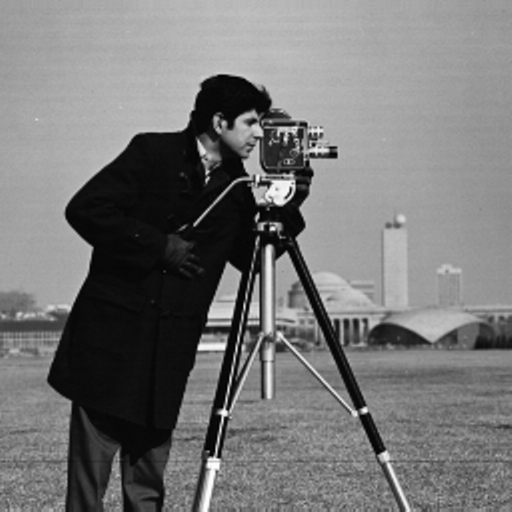
\includegraphics[scale=0.2]{slides/experiments/target-image/cameramen_512x512.png}
\caption{Camera 512x521 target image}
\end{figure}

\column{0.5\textwidth}
\begin{table}
\begin{tabular}{ll}
\hline
          Image Feature & Value \\
\hline
       name &      Camera \\
      shape &  (512, 512) \\
  size\_byte &      262144 \\
 image\_band &        (L,) \\
\hline
\end{tabular}
\caption{Camera Image Characteristics }
\end{table}

\end{columns}
Camera Image, which is a picture where a man was shoted while he was recoding via camera located on a top of tripod.
\end{frame}